\documentclass[conference]{IEEEtran}
\usepackage{amsmath,amssymb,array,graphicx,url,fancyhdr}
\fancypagestyle{firstpage}{\fancyhf{}\renewcommand{\headrulewidth}{0pt}\fancyfoot[C]{\parbox{\textwidth}{\footnotesize AI coding assistants were used for coding and making graphs in this study. The authors take responsibility for the study and its contents.}}}
\setlength{\emergencystretch}{2em}
\renewcommand{\arraystretch}{1.12}
\setlength{\tabcolsep}{4pt}
\newcolumntype{L}[1]{>{\raggedright\arraybackslash}p{#1}}
\newcommand{\code}[1]{\texttt{#1}}
% Generated only from audited measured results.
\newcommand{\OnlineRuns}{840}
\newcommand{\TotalProcesses}{2,712}
\newcommand{\TotalRows}{477,096}
\newcommand{\UsefulInstances}{420,000}
\newcommand{\BestFixedArm}{SS}
\newcommand{\PriorWall}{35.97}
\newcommand{\PriorCPU}{83.89}
\newcommand{\AbstractResults}{Four-candidate screening saves 65.0\% of tuning wall time and 65.9\% of tuning CPU time, with a geometric mean payload penalty of 10.2\% to the same-block empirical best. Its additional payload loss relative to full search's chosen schedule is -1.1\% (95\% CI -3.3\%--0.9\%). For 50 useful executions and an available prior, its total-cost ratio is 1.379 relative to full search (95\% CI 1.329--1.435), where ratios above one favor screening. With calibration counted as useful work, the four-candidate wall ratios are 0.970 at 50 executions and 1.000 at 500, limiting the savings claim to the extra-calibration operating mode. }
\newcommand{\SelectionResults}{Guided 2, Guided 4, and Guided 8 save 82.4\%, 65.0\%, and 31.9\% of tuning wall time, respectively. Their corresponding CPU savings are 83.2\%, 65.9\%, and 32.6\%. Prior-only selection saves 91.1\% wall time and 92.5\% CPU time. These are paired geometric cost ratios over complete tuning phases, not ratios of median milliseconds.}
\newcommand{\QualityResults}{Guided 4's geometric mean payload loss is 10.2\% (95\% CI 7.5\%--13.3\%). It retains 90.7\% of reference speed. Relative to the schedule actually selected by Full 12, its extra payload loss is -1.1\% (95\% CI -3.3\%--0.9\%). Its payload is within 5\% in 44.2\% of runs and within 10\% in 64.2\%. Full search itself has a geometric residual of 11.4\%, illustrating the gap between a finite noisy sweep and an independent best-arm reference.}
\newcommand{\DeploymentResults}{Guided 4's wall-cost ratios at horizons 10, 50, 100, and 500 are 2.014, 1.379, 1.200, 1.053. At 50 executions the CPU-cost ratio is 1.384 (95\% CI 1.335--1.440); at 500 it is 1.053. Ratios above one indicate lower total cost for screening.}
\newcommand{\WorthResults}{At 50 useful executions, 44.2\% of Guided 4 runs satisfy (95\% cluster-bootstrap interval 27.5\%--60.8\%) all three conditions of lower wall cost, lower CPU cost, and at most 5\% payload loss; with a 10\% tolerance this rises to 64.2\%. At 500 executions the corresponding rates are 42.5\% and 60.0\%.}
\newcommand{\CrossoverResults}{For Guided 4, 64 of 120 paired runs have both a tuning saving and a positive payload mean gap to full search. Their median estimated finite crossover is 935 useful executions. This summarizes only runs with a positive gap; it is not a universal operating cutoff.}
\newcommand{\AmortizationResults}{For Guided 4 at horizon 50, the estimated break-even is 488 deployments for wall time and 409 for CPU time. At horizon 500 the estimates are 531 and 448, respectively. When both resources matter, the larger finite count is the relevant lower bound.}
\newcommand{\SensitivityResults}{Under the cross-fitted reference, Guided 4's geometric payload loss becomes -1.7\%; its within-5\% and within-10\% rates become 85.0\% and 92.5\%. The difference from the primary reference quantifies sensitivity to choosing a minimum among noisy same-block timings.}
\newcommand{\ControlResults}{Random 4 has a geometric payload loss of 11.2\% and a horizon-50 wall-cost ratio of 1.403. The trained fixed arm has a loss of 10.2\% and ratio 1.704, with no online calibration. Thus the value of prediction must be considered alongside the simpler ways to spend less on search.}
\newcommand{\DecisionResults}{For the four-candidate policy, the measured exchange is 65.0\% less tuning wall time and 65.9\% less tuning CPU time for 10.2\% aggregate residual payload loss. Its horizon-50 total wall ratio is 1.379, whereas its horizon-500 ratio is 1.053. These measurements make the trade-off explicit; the tolerance hit rate and prior cost determine whether it is acceptable for a particular deployment.}
\newcommand{\ConclusionResults}{On the measured four-core system, Guided 4 avoids two thirds of calibration evaluations and saves 65.0\% tuning wall time and 65.9\% tuning CPU time. Its geometric payload penalty is 10.2\%. For an available prior, its total wall-cost ratio is 1.379 at 50 useful executions and 1.053 at 500. Prior acquisition and tail losses remain part of the decision rather than being hidden costs. The separate equal-useful-work ratios of 0.970 and 1.000 do not establish an in-situ benefit. }
\newcommand{\InsituRuns}{432}
\newcommand{\InsituInstances}{118,800}
\newcommand{\InsituResults}{For 50 equal useful executions, Guided 4's wall-cost ratio is 0.970 (95\% CI 0.933--0.999) and its CPU-cost ratio is 0.970 (95\% CI 0.932--1.001). For 500 equal useful executions, Guided 4's wall-cost ratio is 1.000 (95\% CI 0.987--1.013) and its CPU-cost ratio is 1.001 (95\% CI 0.987--1.014).}
\newcommand{\InsituDecision}{the four-candidate wall-cost ratios are 0.970 at 50 useful calls and 1.000 at 500. These do not establish a time/CPU saving from reduced search in that mode. Avoided candidate tests cannot be counted as avoided necessary executions; the primary extra-calibration savings apply only when calibration is additional work.}

\title{Budgeted OpenMP Scheduling Selection:\\
Time, Compute, and Execution-Quality Trade-offs}
\author{\IEEEauthorblockN{Shaan Chopra, Mrinal Dhami, and Aniket Verma}
\IEEEauthorblockA{School of Computer Science and Engineering\\
Manipal Institute of Technology\\
Group 3: 240905140, 240905026, 240905156}}
\begin{document}
\maketitle
\thispagestyle{firstpage}
\begin{abstract}
Finding the fastest loop scheduler is useful only when the improvement repays
the cost of finding it. We investigate this exchange for OpenMP scheduling:
how much tuning time and CPU consumption can be avoided by accepting a small
loss in subsequent execution quality? A model trained on separate inputs ranks
12 LB4OMP schedulers. Budgeted screening measures only two, four, or eight
candidates before committing; prediction-only, random screening, a trained
fixed scheduler, and full 12-candidate search provide controls. We separately
measure calibration cost, post-selection payload quality, and complete
tuning-plus-useful-execution cost. The fresh experiment comprises
\OnlineRuns{} policy runs on 24 scenarios from three workload families, with
five randomized blocks and directly measured process CPU seconds.
\AbstractResults{}
The paper reports the complete budget--quality frontier, independent
best-arm references, uncertainty, finite-horizon effects, and the number of
deployments needed to amortize the prior. The result is a conditional answer
to when reduced search is worthwhile, rather than a claim that a cheap
selector must outperform the best scheduler itself.
\end{abstract}
\begin{IEEEkeywords}
OpenMP, algorithm selection, tuning budget, CPU time, near-optimal scheduling,
amortization, performance--cost trade-off.
\end{IEEEkeywords}

\section{Introduction}

An OpenMP scheduler assigns loop iterations to threads. Its execution quality
depends on load imbalance, dispatch overhead, locality, and the current
machine. Choosing the fastest scheduler can require executing the loop under
several alternatives. That search is itself work. When an application is
short, the time spent comparing schedules can exceed the time saved by the
best schedule afterward.

The relevant engineering objective is therefore not always minimum
post-selection loop time. An application may prefer a scheduler that is
slightly slower per execution if it is substantially cheaper to identify.
For example, avoiding 24 calibration executions can be useful even if the
selected scheduler loses a few percent of throughput. Whether it is useful
depends on the calibration cost, the execution horizon, the quality gap, and
whether an offline prior must be paid for.

We study this decision directly. A trained model ranks the 12 schedulers in
LB4OMP. Small candidate budgets restrict measurement to promising alternatives
before committing to a fixed schedule. We compare the saved search time and
process CPU seconds with the residual loss relative to an independently
measured best fixed scheduler. Full search is the expensive comparator for
tuning cost; the empirical best scheduler is the reference for execution
quality. These roles are distinct.

This study follows an earlier local experiment that evaluated continuously
updating bandits over 500 useful loop instances and did not establish an
overall speed advantage. The present work asks a different question, uses
fresh test inputs, separates calibration from useful execution, and directly
measures CPU time. It is not a re-labeling of the earlier measurements.

Our research questions are:

\begin{enumerate}
\item How much calibration wall time and process CPU time does a restricted
candidate budget save relative to a full 12-scheduler sweep?
\item What execution-speed penalty remains after the cheaper search, and how
often does it stay within 5\% or 10\% of the empirical best reference?
\item For which useful-execution horizons does the tuning saving outweigh that
penalty, and how many deployments amortize the offline prior?
\end{enumerate}

The contributions are an explicit cost--quality formulation, an implemented
budgeted selector in native C++, a new directly instrumented experimental
corpus, and a deployment decision analysis including unfavorable cases.
We claim neither a new bandit algorithm nor a guarantee of optimal scheduling.

\section{Background and Positioning}

OpenMP exposes standard schedule choices for shared-memory loops
\cite{openmp}. LB4OMP extends LLVM's OpenMP runtime with additional dynamic
and adaptive schedulers \cite{lb4omp}. Auto4OMP adds automated selection and
an expert chunk-size calculation \cite{auto4omp}. Our experiment reuses those
implementations and the expert chunk rule; it changes the budget spent
identifying a scheduler.

M\"uller Kornd\"orfer et al. compare expert and reinforcement-learning
selectors across six applications and three systems \cite{comparative}.
Their 12-scheduler explore-first formulation considers 144 ordered
state--action combinations. They identify exploration cost and reward choice
as important practical issues. This motivates reducing selection effort, but
does not require beating an offline best scheduler in subsequent loop speed.
We instead expose the quality lost per unit of search work avoided.

Algorithm selection distinguishes an algorithm that is best on average from
a virtual best choice for each instance. Tornede et al. note that exhaustive
evaluation is costly and that feature-computation time must be included in
runtime objectives \cite{meta}. This distinction applies directly here:
a model that identifies a good schedule cheaply can be useful without
identifying the fastest one every time.

Contextual bandits use context to predict action rewards \cite{linucb}.
Warm-start methods incorporate earlier information into their initial models
\cite{oetomo}. We use a fitted disjoint linear model originating from that
framework to rank candidates, then stop exploration at a declared budget.
There is no online regret theorem or claimed confidence guarantee for this
screening heuristic. The contribution is the measured budget--quality exchange.

The workload families follow the ideas of Mandelbrot, STREAM-style vector
arithmetic, and sorted-adjacency triangle counting \cite{stream,gap}.
Our kernels are original compact implementations, not the reference STREAM
or GAP programs. Uncertainty is estimated at input-configuration level,
following the need to distinguish repetitions from independent experiments
in systems benchmarking \cite{kalibera}.

\section{Cost--Quality Formulation}

Let $\mathcal A$ contain the 12 schedulers. A selector $m$ spends tuning time
$S_m$ to commit to $a_m\in\mathcal A$. Afterward it executes $H$ useful loop
instances. With a reusable prior costing $C_{\mathrm{prior}}$ and shared
across $R$ deployments, the wall-time objective is
\begin{equation}
 J_m^{\mathrm{wall}}(H,R)=
 \frac{C_{\mathrm{prior}}^{\mathrm{wall}}}{R}
 +S_m^{\mathrm{wall}}+\sum_{t=1}^{H}T_t^{\mathrm{wall}}(a_m).
 \label{eq:objective}
\end{equation}
An analogous expression uses measured process CPU seconds. A selector without
an offline prior, such as random screening or full search, has
$C_{\mathrm{prior}}=0$ in this operational comparison. A fixed arm selected
from the training campaign also uses offline information, so its acquisition
cost must be charged when that information is not already available.

For an empirical best fixed-arm reference $T^*$, the residual payload slowdown
is
\begin{equation}
 \ell_m=\frac{\widetilde T(a_m)}{\widetilde T^*}-1,
 \qquad \rho_m=\frac{\widetilde T^*}{\widetilde T(a_m)}
              =\frac{1}{1+\ell_m},
 \label{eq:quality}
\end{equation}
where tildes denote medians of independent timing observations.
$\rho_m$ is retained speed relative to the reference. For example, a 5\%
runtime penalty retains approximately 95.24\% of the reference speed.
We study the frontier between $S_m$ and $\ell_m$, rather than treating
reference-matching speed as the sole success criterion.

\subsection{When is the exchange worthwhile?}

Let $F$ denote full search. For a cached prior, restricted selection is faster
over horizon $H$ whenever
\begin{equation}
 S_F-S_m > \sum_{t=1}^{H}\left[T_t(a_m)-T_t(a_F)\right].
 \label{eq:worth}
\end{equation}
Under stationary mean payload times and a positive gap
$\Delta T=\bar T(a_m)-\bar T(a_F)>0$, the estimated crossover is
\begin{equation}
 H^*=\frac{S_F-S_m}{\Delta T}.
 \label{eq:crossover}
\end{equation}
The restricted method benefits shorter executions and loses its advantage
after sufficient repetition. If the measured gap is nonpositive, this model
has no finite crossover favoring full search; that is an empirical case,
not a promise about future executions. Finite search may choose a noisy winner,
so full search is not assumed to be a perfect Oracle.

With an unpaid prior, the left side of Eq.~\ref{eq:worth} is reduced by
$C_{\mathrm{prior}}/R$. If $d(H)$ is the mean measured per-deployment saving,
the minimum estimated reuse count is
\begin{equation}
 R_{\min}(H)=\left\lceil\frac{C_{\mathrm{prior}}}{d(H)}\right\rceil
 \quad\text{when }d(H)>0.
 \label{eq:reuse}
\end{equation}
If $d(H)\leq0$, repeated reuse does not amortize the prior for that comparison.
Wall and CPU break-even counts are calculated separately.
They are point estimates; an interval for mean savings that crosses zero
does not support a confident finite amortization claim.

\subsection{Two meanings of exploration}

The primary experiment uses \emph{tune-then-run}: calibration executions are
additional evaluations before the $H$ useful loop instances. This is suitable
for repeated kernels with representative trial inputs or a calibration phase
whose results are not counted as application progress. It is the setting in
which fewer evaluations directly avoid extra work.

In an in-situ selector, exploratory loop instances may already advance the
application. Removing 24 trials does not then remove 24 required useful
executions. Its cost is the excess time of those trials relative to a
deployment schedule, not their full execution time. The present measurements
do not establish equivalent savings in that setting. This semantic distinction
is necessary to interpret the proposed trade-off.

\section{Budgeted Candidate Screening}

\subsection{Prior and context}

The context is
$x=[1,\log_2N,\log_2P,\log_2T_0,L_0,V_0]^\top$, where $T_0$ is the median
of three STATIC probes, $L_0$ is median finish-time imbalance, and $V_0$ is
median coefficient of variation of thread finish times. Thread finishes are
measured relative to parallel-region start, so launch and arrival effects
are included. Non-intercept features are standardized using training data.

For arm $a$, a ridge model is initialized using training scenario contexts and
normalized log-time rewards:
\begin{align}
 r_{i,a}&=\operatorname{clip}\left(
 -\frac{\log(T_{i,a}/T_{i,\mathrm{STATIC}})}{\log4},-1,1\right),\\
 A_a&=\lambda I+w\sum_i x_ix_i^\top,\\
 b_a&=w\sum_i x_i r_{i,a},\qquad
 \hat\theta_a=A_a^{-1}b_a.
\end{align}
Arms are ranked by $x^\top\hat\theta_a$. The inherited values
$w=0.25$ and $\lambda=1$ are frozen from the preceding study's training-only
validation. A stored exploration coefficient of 0.025 is not used in the
greedy ranking. This paper tests fixed measurement budgets, not continuously
updating LinUCB.

\subsection{Budget definitions and controls}

Table~\ref{tab:policies} defines the seven treatments. The three STATIC probes
also supply a measured safety candidate. For Guided $q$, we test the top
$q-1$ predicted non-STATIC arms three times each, then choose the minimum
observed median among those arms and STATIC. The cap is an explicit number
of candidates, not a claim that each candidate has equal execution cost.

\begin{table*}[t]
\centering\small
\caption{Policies and extra calibration executions. Model ranking and loading
cost are included in tuning time where used.}
\label{tab:policies}
\begin{tabular}{lrrL{8.2cm}}
\hline
Policy & Candidates tested & Evaluations & Commitment rule\\
\hline
Best fixed & 0 & 0 & Training-best arm; no online tuning.\\
Prior only & 1 & 3 & Three STATIC probes; choose the prior's best predicted arm,
which may not itself have been measured online.\\
Guided 2 & 2 & 6 & STATIC plus the top predicted non-STATIC arm.\\
Guided 4 & 4 & 12 & STATIC plus three predicted candidates.\\
Guided 8 & 8 & 24 & STATIC plus seven predicted candidates.\\
Random 4 & 4 & 12 & STATIC plus three uniformly sampled non-STATIC arms.\\
Full 12 & 12 & 36 & All arms, three observations each; minimum median.\\
\hline
\end{tabular}
\end{table*}

Full search saves no calibration evaluations relative to itself. Guided 4
reduces the count by two thirds; Prior only reduces it by 91.7\%. These exact
count reductions do not imply equal wall-time or CPU reductions. Actual
selection costs are measured, and residual payload quality is evaluated
independently after commitment. No method continues switching during payload.

\section{Implementation and Experimental Protocol}

\subsection{Native implementation and CPU accounting}

The C++ implementation reuses the previously audited workload and scheduling
code. It adds explicit probe, tuning, and payload phases. Wall time uses a
monotonic clock. CPU time uses \code{CLOCK\_PROCESS\_CPUTIME\_ID}, which
accounts for CPU time consumed by all threads in the process \cite{clock}.
It includes active waiting within the OpenMP runtime during the measured
phase. It is neither energy consumption nor a count of FLOPs or instructions.

Each timed loop records wall seconds, process CPU seconds, scheduler ID,
kernel elapsed time, imbalance, and variation. Prefix snapshots record actual
wall and CPU costs for the first 10, 50, 100, and 500 useful executions.
These are measured prefixes of a committed run, not independently repeated
experiments at four horizons. Model deserialization and ranking are charged
to tuning for prior-based methods. Common input construction and two STATIC
warm-up executions are excluded from deployment cost for all treatments.
Whole-process elapsed and CPU costs are also recorded.

The machine is an AMD Ryzen 5 7235HS with four physical cores/eight logical
CPUs and approximately 7.6\,GiB visible RAM under WSL2 Linux
\code{6.6.87.2}. Clang 16.0.6 uses \code{-O3 -std=c++17 -fopenmp
-ffp-contract=off}. LB4OMP commit
\code{b9d25eca7265a4b5b3a675a1765d489775847938} has a portability-only
initialized-array-to-vector patch. Threads are pinned to physical-core
representatives $0,2,4,6$; the active wait policy and 200\,ms block time are
fixed. Dynamic teams are disabled. Host activity, thermal state, and turbo
are uncontrolled and limit the precision of small differences.

The expert chunk rule is enabled for every treatment. In the pinned runtime,
it can override STATIC's chunk size as well; STATIC therefore uses cyclic
expert-sized chunks rather than a single contiguous block per thread.
The scheduling portfolio is STATIC, SS, TSS, AutoLLVM, GSS, mFAC2,
Static Steal, AWF-B, AWF-C, AWF-D, AWF-E, and mAF.

\subsection{Fresh training and unseen test inputs}

We collect fresh calibration measurements for the original training
configurations, seeds 0 and 1, at two and four threads. For every scenario,
all 12 arms run in three separate processes. Each process has three STATIC
probe observations and 20 observations of the target arm. One median label
per scenario/arm fits the model, rather than treating individual loop rows
as independent prior evidence. This is 432 calibration processes.
The training-selected fixed arm is \BestFixedArm{}.

New test configurations use seeds 4--7. They are disjoint from both training
and the preceding paper's seeds 2 and 3. Table~\ref{tab:inputs} lists all sizes.
Each configuration runs at $P\in\{2,4\}$, yielding 24 scenarios and 12 input
configuration clusters. All arms and treatments within one scenario use
identical deterministic inputs and produce the same useful outputs.

\begin{table*}[t]
\centering\small
\caption{New held-out configurations, each measured at two thread counts.}
\label{tab:inputs}
\begin{tabular}{lrrrr}
\hline
 & Seed 4 & Seed 5 & Seed 6 & Seed 7\\
\hline
Mandelbrot pixels & 36,864 & 57,600 & 20,736 & 43,264\\
Maximum pixel iterations & 192 & 216 & 240 & 264\\
Triad elements & 524,288 & 655,360 & 458,752 & 917,504\\
Triangle vertices & 768 & 1,792 & 1,280 & 1,920\\
\hline
\end{tabular}
\end{table*}

Mandelbrot uses a square row-major grid, a real-coordinate shift of
$0.025(\mathrm{seed}\bmod4)$, and a seed-dependent iteration cap.
Triad evaluates $a_i=b_i+3c_i$ on three double arrays. The graph generator
makes $24N$ undirected edge proposals using a seeded \code{mt19937}; one third
have an endpoint in a hub-biased prefix, while others are uniform. It removes
self-edges and duplicates, orients by vertex ID, and counts triangles using
sorted-neighbor intersections. Graph construction is outside tuning and
payload timing. These small synthetic inputs do not establish performance
on large real graphs or production HPC applications.

\subsection{Randomized blocks and independent references}

The frozen protocol declares five blocks. Every block shuffles 168 policy
processes and 288 independent fixed-arm reference processes. Each reference
process measures 25 payload executions of one arm after the common warm-ups;
it does not provide labels to the selector. Reference and policy jobs execute
sequentially to avoid concurrent benchmark contention. Source, binary, model,
protocol, raw CSV, and summary hashes are recorded.

For scenario $s$ and block $b$, the primary empirical quality reference is
\begin{equation}
 \widetilde T^*_{s,b}=\min_{a\in\mathcal A}
 \operatorname{median}_{j=1}^{25}T_{s,b,a,j}^{\mathrm{reference}}.
\end{equation}
The selected policy's quality uses its median over 500 post-selection payload
observations in a separate process. These loop observations are not treated
as independent experimental replications. A minimum over noisy reference medians is optimistic. We do
not treat this value as a known mathematical optimum, and negative observed
slowdowns are retained as noise rather than clipped.

A cross-fitted sensitivity selects the reference arm using the other four
blocks, then evaluates that arm's time in the held-out block. This separates
selecting the reference arm from measuring its held-out time. It is an
analysis-only addition recorded during the first block, before aggregate
test outcomes were examined. Both reference definitions are reported.

\subsection{Correctness and uncertainty}

The shared kernels passed a scheduler-coverage test for all 12 arms at both
thread counts and an independent cubic triangle-count check on a tiny graph.
Every new process compares its final parallel checksum with a serial
evaluation. Candidate counts, selected-arm identity, phase lengths, and raw
hashes are audited. Repeated identical input means final-output checks alone
do not certify each intermediate iteration; coverage is tested separately.

Paired effects compare policies within the same scenario and block.
We report geometric mean ratios and 95\% bootstrap intervals from 10,000
resamples of the 12 input configurations, with paired observations resampled
inside each cluster. Both thread counts belong to their common input cluster.
Individual loop observations and horizon prefixes are not independent
replications. Acceptance rates within 5\% and 10\% are descriptive empirical
frequencies, not validated deployment guarantees.

\section{Results: The Search--Quality Frontier}

The primary corpus contains \TotalProcesses{} audited processes and
\TotalRows{} logged loop observations, including calibration and references.
There are \OnlineRuns{} policy runs and \UsefulInstances{} useful online
executions. All process output checks passed. The following results separate
selection saving, payload quality, and complete deployment cost.

\subsection{Calibration time and CPU savings}

\begin{table*}[t]
\centering\small
\caption{Measured tuning cost relative to Full 12. Savings are paired geometric effects; median wall milliseconds are descriptive.}
\label{tab:selection}
\begin{tabular}{lrrrr}
\hline
Policy & Evaluations & Median wall (ms) & Wall saved (\%) & CPU saved (\%)\\
\hline
Best fixed & 0 & 0.01 & 100.0 & 100.0 \\
Prior only & 3 & 8.24 & 91.1 & 92.5 \\
Guided 2 & 6 & 16.45 & 82.4 & 83.2 \\
Guided 4 & 12 & 32.16 & 65.0 & 65.9 \\
Guided 8 & 24 & 63.48 & 31.9 & 32.6 \\
Random 4 & 12 & 30.91 & 67.2 & 67.7 \\
Full 12 & 36 & 91.14 & 0.0 & 0.0 \\
\hline
\end{tabular}
\end{table*}

\SelectionResults{}
The evaluation-count reductions are fixed by policy; measured wall and CPU
reductions need not equal them because candidates have different costs and
model loading adds overhead. CPU seconds include runtime active waiting,
so they quantify process resource consumption under the stated runtime
configuration, not an architecture-independent operation count.

\subsection{Residual scheduling quality}

\begin{table*}[t]
\centering\small
\caption{Independent payload-quality measurements. Geometric mean and 90th-percentile residual slowdowns are relative to the same-block empirical best. Acceptance rates are observed run fractions.}
\label{tab:quality}
\begin{tabular}{lrrrr}
\hline
Policy & Mean loss (\%) & P90 loss (\%) & Within 5\% & Within 10\%\\
\hline
Best fixed & 10.2 & 32.9 & 40.0 & 65.8 \\
Prior only & 10.4 & 32.4 & 41.7 & 66.7 \\
Guided 2 & 9.9 & 33.1 & 36.7 & 72.5 \\
Guided 4 & 10.2 & 31.2 & 44.2 & 64.2 \\
Guided 8 & 10.4 & 26.8 & 38.3 & 67.5 \\
Random 4 & 11.2 & 35.2 & 35.0 & 62.5 \\
Full 12 & 11.4 & 36.0 & 40.8 & 65.8 \\
\hline
\end{tabular}
\end{table*}

\QualityResults{}
Figure~\ref{fig:frontier} places measured tuning saving and residual payload
loss on separate axes. A useful policy moves toward lower search cost while
keeping its payload loss within an application's declared tolerance.

\begin{figure}[t]
\centering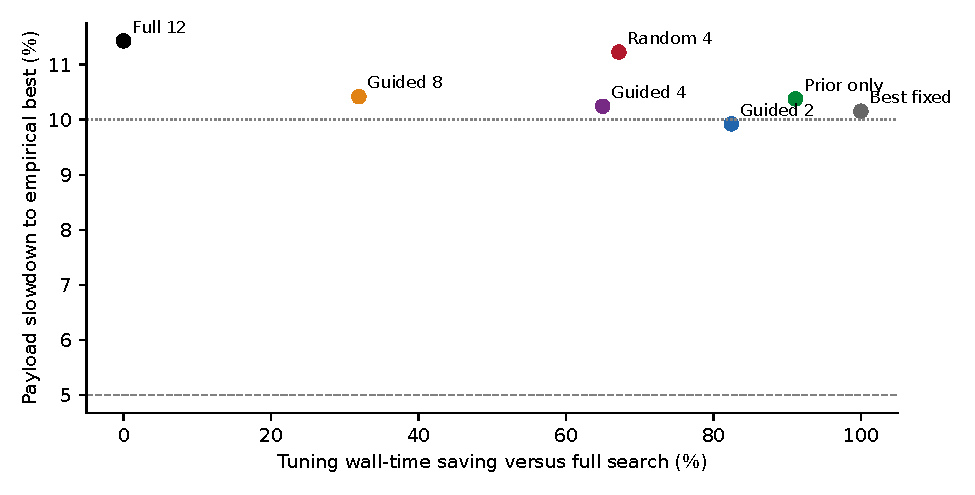
\includegraphics[width=\linewidth]{figures/tradeoff.pdf}
\caption{Measured tuning wall-time saving versus residual payload slowdown.
Points are geometric aggregate effects over all scenarios and blocks.
Horizontal guides mark 5\% and 10\% slowdown tolerances; they are application
preferences, not statistical confidence limits.}
\label{fig:frontier}
\end{figure}

\subsection{Does the saved tuning work repay the quality loss?}

\begin{table*}[t]
\centering\small
\caption{Total wall-cost ratios: Full 12 cost divided by policy cost, including tuning and H useful executions. Values above one favor the policy. Prior acquisition is excluded here and charged separately.}
\label{tab:deployment}
\begin{tabular}{lrrrr}
\hline
Policy & H=10 & H=50 & H=100 & H=500\\
\hline
Best fixed & 4.556 & 1.704 & 1.360 & 1.084 \\
Prior only & 3.453 & 1.621 & 1.333 & 1.081 \\
Guided 2 & 2.795 & 1.544 & 1.294 & 1.069 \\
Guided 4 & 2.014 & 1.379 & 1.200 & 1.053 \\
Guided 8 & 1.327 & 1.166 & 1.104 & 1.032 \\
Random 4 & 2.128 & 1.403 & 1.226 & 1.050 \\
Full 12 & 1.000 & 1.000 & 1.000 & 1.000 \\
\hline
\end{tabular}
\end{table*}

\DeploymentResults{}
These ratios include calibration and the same number of useful executions.
They assume the prior is already available; its acquisition is charged in
the following subsection. A method can save most tuning work yet lose its
total-cost advantage over long horizons when its committed arm is slower.

\begin{figure}[t]
\centering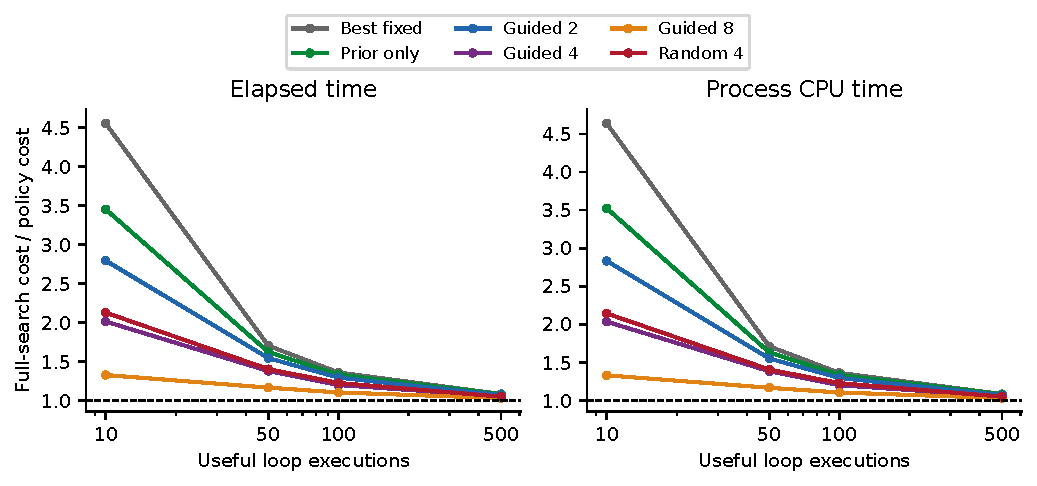
\includegraphics[width=\linewidth]{figures/horizons.pdf}
\caption{Full-search deployment cost divided by each policy's deployment
cost, including tuning. Values above one favor the restricted policy.
The left panel measures elapsed time; the right measures process CPU time.
Horizon prefixes come from the same committed runs.}
\label{fig:horizons}
\end{figure}

\WorthResults{}
The joint criterion requires lower total wall time, lower total CPU time,
and payload loss within the stated tolerance in the same observed run.
It is more demanding than reporting either tuning saving or quality alone.
\CrossoverResults{}

\subsection{The cost of acquiring the prior}

Fresh operational calibration and fitting cost \PriorWall{} wall seconds and
\PriorCPU{} process CPU seconds. Calibration includes complete subprocess
costs---input construction, warm-ups, timing, correctness validation, and
output---while fitting includes loading measurements, computing statistics,
and serializing the model. Build time, Python import startup, and the earlier
research campaign that chose inherited hyperparameters are excluded. The
reported cost therefore describes operational reuse of the fixed recipe,
not the entire cost of inventing the method.

\AmortizationResults{}
Equation~\ref{eq:reuse} uses arithmetic mean per-deployment savings because
actual seconds, rather than logarithmic ratios, repay an upfront expense.
The reuse counts are estimates for the measured workload mixture. If the
mean saving is nonpositive, no finite count is reported. A prior available
from an existing deployment and a newly acquired prior are materially
different operating conditions.

\subsection{Reference sensitivity and simple alternatives}

\SensitivityResults{}
The cross-fitted reference reduces same-block winner selection bias but is
not a guarantee of the true optimum either. Timing noise, family similarity,
and the limited number of configurations still affect both estimates.

\ControlResults{}
A zero-online-tuning fixed arm can be a strong choice when the training
distribution is representative. Random screening tests whether candidate
count alone explains a favorable trade-off. These controls prevent
attributing every saved evaluation to contextual prediction.

\begin{table*}[t]
\centering\small
\caption{Four-candidate screening by workload family: calibration wall saving, payload loss to the empirical best, and complete deployment wall-cost ratios. Each family contains four input configurations at two thread counts.}
\label{tab:family}
\begin{tabular}{lrrrr}
\hline
Family & Tuning saved (\%) & Payload loss (\%) & H=50 ratio & H=500 ratio\\
\hline
Mandelbrot & 64.6 & 7.5 & 1.369 & 1.034 \\
Triad & 63.0 & 11.4 & 1.351 & 1.076 \\
Triangle & 67.2 & 12.0 & 1.418 & 1.050 \\
\hline
\end{tabular}
\end{table*}


\begin{figure}[t]
\centering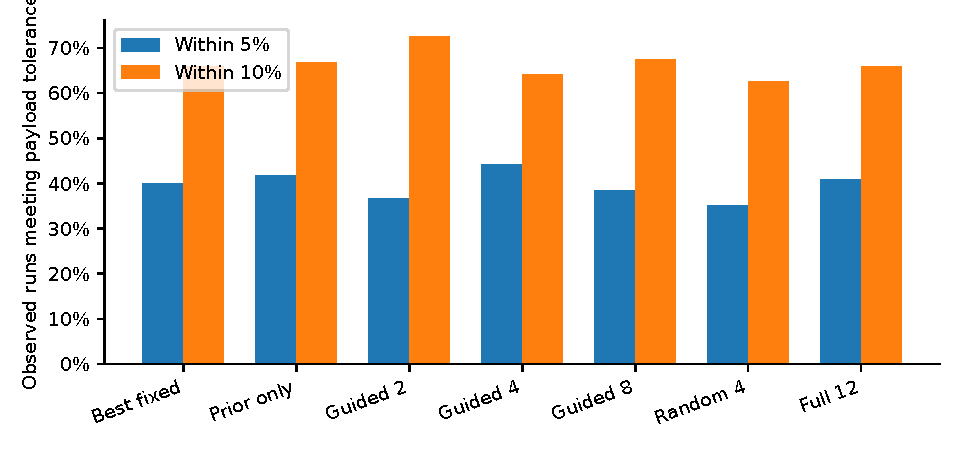
\includegraphics[width=\linewidth]{figures/acceptance.pdf}
\caption{Observed policy runs whose payload median is within 5\% or 10\%
of the independent same-block empirical best. These rates measure execution
quality separately from search saving and do not imply a probabilistic
guarantee for new programs.}
\end{figure}

\subsection{Secondary equal-useful-work experiment}

To examine the original online interpretation directly, we additionally
measure Prior only, Guided 4, and Full 12 with exactly 50 or 500 total useful
executions, counting calibration calls as useful. For $H=50$, Full 12 spends
36 useful calls measuring candidates and then performs 14 committed calls;
Guided 4 spends 12 and then performs 38. Thus both do the same total work.
These are new direct measurements in three randomized blocks on all 24
scenarios, not reconstructed prefixes of the primary experiment.

The executable and fitted model are unchanged. Each native process is given
$H-n_m$ committed payload calls, where $n_m$ is its calibration count, and
we charge the measured tuning and complete payload phases. The additional
experiment was declared during the primary campaign, before aggregate
outcomes were inspected. Its \InsituRuns{} processes contain
\InsituInstances{} useful executions. \InsituResults{}
\begin{table*}[t]
\centering\small
\caption{Secondary equal-useful-work results. Both tuning and committed calls count toward H; cost ratios are Full 12 divided by the policy. All intervals use input-cluster resampling.}
\label{tab:insitu}
\begin{tabular}{lrrrr}
\hline
Policy & H & Wall ratio & Wall 95\% CI & CPU ratio\\
\hline
Prior only & 50 & 0.990 & 0.950--1.026 & 0.991 \\
Guided 4 & 50 & 0.970 & 0.933--0.999 & 0.970 \\
Prior only & 500 & 0.997 & 0.978--1.015 & 0.998 \\
Guided 4 & 500 & 1.000 & 0.987--1.013 & 1.001 \\
\hline
\end{tabular}
\end{table*}


\section{Discussion: Is the Trade-off Worth It?}

\DecisionResults{}

The equal-useful-work experiment qualifies this conclusion for in-situ use:
\InsituDecision{}

The objective is a choice among resource and quality preferences. A user who
accepts a small loss in per-loop speed may prefer cheap screening when the
run is short or the prior is already available. A long, repeated execution
can justify more measurement because its payload dominates the total cost.
An expensive prior acquired for a single short deployment can erase the
online saving. The correct comparison is Eq.~\ref{eq:objective}, with a
declared horizon, tolerance, and reuse assumption.

Our implementation makes budget decisions explicit: measure only a declared
candidate set, stop, and commit. The quality penalty is therefore attributable
to that selection rule and measurement noise, rather than being hidden inside
continuous online exploration. However, candidate count is only a proxy for
resource use. The directly measured wall and CPU costs are the evidence for
saving time and compute in this experiment.

Those savings do not establish that contextual prediction is necessary.
The fixed and random-screening controls also reduce search effort; their
results must remain visible when assessing the learned ranking. Nor does
spending a larger budget ensure a strictly better committed schedule in
every finite noisy run. The measured exchange is about operational cost and
execution quality, not an ordering theorem over candidate counts.

The full sweep may itself choose a noisy winner from only three observations
per arm. Its payload need not match the independent best-arm reference.
This is why we report both a costly feasible search comparator and an
independent execution-quality reference. Near-reference quality with lower
search cost is the target; beating an unavailable zero-cost Oracle is not.

\section{Limitations and Scope}

\textbf{Tuning semantics.} Savings are measured for additional calibration
executions. They do not automatically transfer to in-situ application progress.
The method assumes repeatable representative probes and an input state that
can be reused or restored cheaply. Stateful applications may have additional
copying or reset costs that are absent from these kernels.

\textbf{Machine and workloads.} One four-core WSL2 system and compact
synthetic kernels do not support conclusions about multi-socket HPC, NUMA,
heterogeneous devices, or large real-world graphs. Active waiting affects
CPU consumption. Host activity, frequency, and temperature are uncontrolled.
Training and test inputs belong to the same three families; seed holdout is
not unseen-application generalization.

\textbf{Reference and tolerance.} Finite reference medians and their minimum
are noisy. Threshold rates near 5\% can change under reference uncertainty.
The cross-fitted sensitivity addresses one source of optimism but not all
nonstationarity. No worst-case near-optimality guarantee is claimed.
References contain 25 observations per process, whereas committed policy
quality uses 500. Different run duration can expose cache, adaptive-runtime,
frequency, or thermal transients. We cannot isolate those effects here.
Negative cross-fitted gaps do not show that a policy beats a true optimum;
they show that a finite empirical reference can be outperformed or fluctuate.

\textbf{Prior and policy design.} Hyperparameters are inherited rather than
retuned for this budgeted objective. Three repeats per candidate are fixed.
Rank-based screening can omit a useful arm, and the model's clipped log-time
target is a surrogate rather than an exact total-cost objective. Tolerance
and budget are fixed preferences, not adaptively chosen per deployment.

\textbf{Statistical and cost scope.} There are 12 input clusters, not hundreds
of thousands of independent experiments. Prefixes share observations.
Crossover and amortization extrapolate stationary means. Operational training
cost excludes method-development effort. CPU time measures consumed processor
time, including waiting, and cannot establish energy or instruction savings.

\section{Conclusion}

We evaluate OpenMP scheduler selection as a budget--quality decision.
The implementation directly measures the work spent choosing a schedule and
the execution quality left after that choice. \ConclusionResults{}
The practical decision should declare a useful-execution horizon, a tolerated
payload loss, whether calibration is extra work, and how the prior is paid
for. Reporting those conditions makes a near-best scheduling policy useful
on its own terms without requiring it to be the fastest scheduler.

\begin{thebibliography}{99}
\bibitem{openmp} OpenMP Architecture Review Board. OpenMP Application
Programming Interface, Version 5.2 (2021).
\url{https://www.openmp.org/specifications/}
\bibitem{lb4omp} J.H. M\"uller Kornd\"orfer, A. Eleliemy, A. Mohammed,
F.M. Ciorba. LB4OMP: A Dynamic Load Balancing Library for Multithreaded
Applications. IEEE TPDS 33(4), 830--841 (2022).
\url{https://doi.org/10.1109/TPDS.2021.3107775}
\bibitem{auto4omp} A. Mohammed, J.H. M\"uller Kornd\"orfer, A. Eleliemy,
F.M. Ciorba. Automated Scheduling Algorithm Selection and Chunk Parameter
Calculation in OpenMP. IEEE TPDS 33(12), 4383--4394 (2022).
\url{https://doi.org/10.1109/TPDS.2022.3189270}
\bibitem{comparative} J.H. M\"uller Kornd\"orfer, A. Mohammed, A. Eleliemy,
Q. Guilloteau, R. Krummenacher, F.M. Ciorba. A Comparative Study of OpenMP
Scheduling Algorithm Selection Strategies. IEEE Access 13, 151216--151234
(2025). \url{https://doi.org/10.1109/ACCESS.2025.3602234}
\bibitem{meta} A. Tornede, L. Gehring, T. Tornede, M. Wever,
E. H\"ullermeier. Algorithm Selection on a Meta Level. Machine Learning 112,
1253--1286 (2023). \url{https://doi.org/10.1007/s10994-022-06161-4}
\bibitem{linucb} L. Li, W. Chu, J. Langford, R.E. Schapire.
A Contextual-Bandit Approach to Personalized News Article Recommendation.
In WWW, 661--670 (2010). \url{https://doi.org/10.1145/1772690.1772758}
\bibitem{oetomo} B. Oetomo, R.M. Perera, R. Borovica-Gajic,
B.I.P. Rubinstein. Cutting to the Chase with Warm-Start Contextual Bandits.
Knowledge and Information Systems 65, 3533--3565 (2023).
\url{https://doi.org/10.1007/s10115-023-01861-2}
\bibitem{stream} J.D. McCalpin. STREAM: Sustainable Memory Bandwidth in
High Performance Computers. \url{https://www.cs.virginia.edu/stream/}
\bibitem{gap} S. Beamer, K. Asanovi\'c, D. Patterson. The GAP Benchmark
Suite. arXiv:1508.03619 (2015). \url{https://arxiv.org/abs/1508.03619}
\bibitem{kalibera} T. Kalibera, R. Jones. Rigorous Benchmarking in Reasonable
Time. ISMM, 63--74 (2013). \url{https://kar.kent.ac.uk/33611/}
\bibitem{clock} Linux man-pages project. \code{clock\_gettime(3)}:
clock and process CPU-time definitions.
\url{https://man7.org/linux/man-pages/man3/clock_gettime.3.html}
\end{thebibliography}
\end{document}
